% Generated only after the full independent 15,000-response audit.
\begin{figure*}[t]
\centering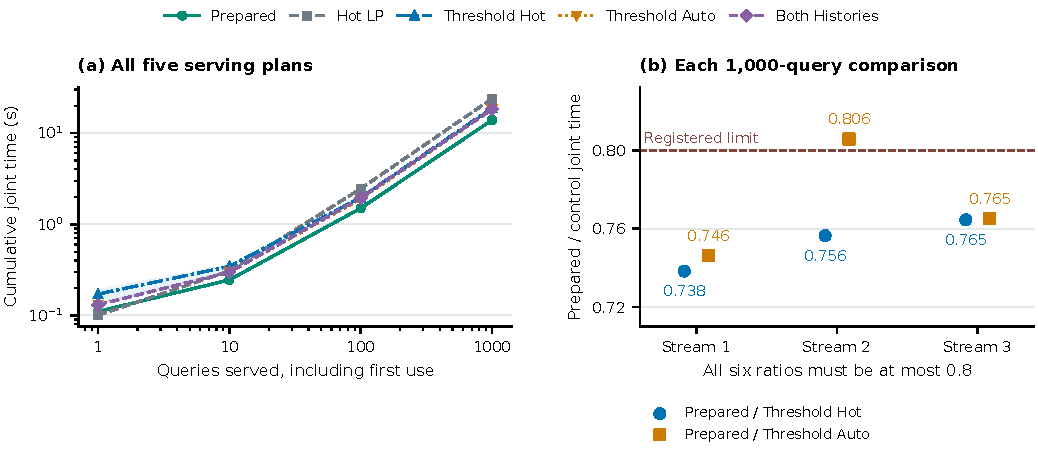
\includegraphics[width=\textwidth]{figures/primary_aligned_v3.pdf}
\caption{Matched execution on the original 512-cell, 1,000-query streams. (a) Joint producer and persistent-receiver time, including initialization; lines are medians and bands are minima/maxima over three paired streams, not confidence intervals. Both axes are logarithmic. (b) All six primary joint-cost ratios; one exceeds the registered $.8$ limit. Every plan answers every query true in this constructed workload.}
\label{fig:primary-aligned}
\end{figure*}
\begin{table}[t]
\centering
\caption{Matched 1,000-query costs in seconds: medians of three paired streams. Joint is added within each stream before taking its median; displayed component medians need not sum to it.}
\label{tab:primary-aligned}\begingroup\fontsize{8}{9.5}\selectfont\setlength{\tabcolsep}{3.2pt}
\begin{tabular*}{\columnwidth}{@{\extracolsep{\fill}}lrrr@{}}
\toprule
Plan & Producer & Receiver & Joint\\
\midrule
Prepared & 5.75 & 8.15 & 13.89\\
Hot LP & 9.76 & 14.12 & 23.87\\
Threshold Hot & 10.35 & 8.36 & 18.81\\
Threshold Auto & 10.01 & 8.15 & 18.15\\
Both Histories & 10.11 & 8.19 & 18.30\\
\bottomrule
\end{tabular*}
\endgroup

\end{table}

\textbf{Matched threshold-aware result.} Prepared's joint-cost ratios are 0.738, 0.756, 0.765 against Threshold Hot and 0.746, 0.806, 0.765 against Auto (Fig.~\ref{fig:primary-aligned}, Table~\ref{tab:primary-aligned}). All six comparisons favor Prepared on these sequences; the requirement that every ratio be at most $.8$ still fails. All five plans return 1,000 true answers on each sequence, with no lost decided answer or contradiction. An independent rational implementation validates all 15,000 lower proofs and their exact query/view bindings; no upper proof is returned here. This positive-query workload therefore supports a local cost comparison, not a test of negative decisions or near-threshold ambiguity. The broader threshold grid below supplies those cases. The three sequences do not support a significance claim.

\textbf{Same candidate, different checking work.} Prepared and all three threshold variants solve once per stream, then reuse one dual 999 times. Prepared ranks floating proposals before exact evaluation; the threshold variants first exactly evaluate the zero-dual box bound, then check the last dual, recording 2,000 exact candidate checks. Mean producer verification is 4.59\,s for Prepared versus 8.97/8.65\,s for the two controls; receiver verification is similar. Every threshold plan also pays for one rejected primal proposal, without losing a positive answer. These measured implementation paths explain where work occurs; no controlled ablation assigns the entire saving to one operation. In particular, the eager box check is not required by two-sided semantics. The comparison demonstrates local implementation savings, not an inherent advantage over threshold-aware execution or a benefit from a larger history.
